\section{Fonctionnement statique}
\begin{center}
	 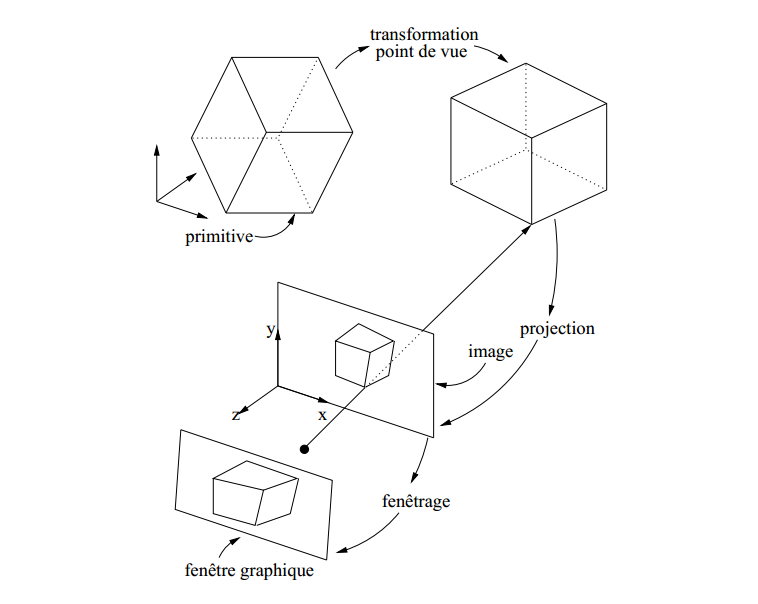
\includegraphics[height=11cm]{img/Fonctionnement}
 \end{center}

La première étape\footnote{http://duriansoftware.com/joe/An-intro-to-modern-OpenGL.-Chapter-1:-The-Graphics-Pipeline.html} est de définir les primitives des objets à dessiner (x,y,z pour chaque Vertex).
OpenGL dessine une image tampon qui sera soit conservée dans la mémoire vidéo de la fenêtre graphique avant d’être affichée, soit une image tampon intermédiaire, on parle alors de double buffering.

La transformation du point de vue sert à la position du plan image. Elle prend en compte la position de la caméra pour se placer correctement autour de l'objet. Ces modifications sont faites à l'aide de matrices. 

Les primitives sont ensuite projetées sur ce plan en fonction des paramètres que l’on a affecté à la projection. Cette projection peut être spécifiée de deux manières. (Voir Projection)

Au final l’image que l’on obtient est redimensionnée en fonction de la taille de la fenêtre graphique . On parle maintenant de pixels et plus de vertex.
\newpage

\subsection{Primitives}
Tout d'abord, il s'agit de définir chaque objet à modéliser, grâce aux primitives précédemment décrites.

Dans le code, chaque primitives est décrite de la manière suivante:


%//////////////////////////////////
%NE PAS TOUCHER A CE TRUC IMMONDE :)
\begin{tabbing}
XXXX\=XXXX\= \kill

\> \verb|glBegin("type_de_primitive");| \\
\> \> glVertex(x,y,x);\\
\> \> . \\
\> \> . On définit chaque vertex en fonction du type de primitive\\
\> \> . \\
\> \> glVertex(x,y,x);\\
\> glEnd();
\end{tabbing}
%NE PAS TOUCHER A CE TRUC IMMONDE :)
%//////////////////////////////////

\subsection{Transformation de point de vue}
La transformation de point de vue consiste en la modification d'une matrice appelée MODELVIEW. Il faut d'abord signaler à OpenGL que l'on veut modifier cette matrice avec la fonction suivante :

\begin{tabbing}
XXXX\= \kill
\> \verb|glMatrixMode( GL_MODELVIEW );|
\end{tabbing}

Ensuite, on charge la matrice identité, ce qui permet de réinitialiser la matrice en cours, puis définit la caméra.

\begin{tabbing}
XXXX\= \kill
\> \verb|glLoadIdentity( );| \\
\> \verb|gluLookAt(eyeX,eyeY,eyeZ,centerX,centerY,centerZ,upX,upY,upZ);|
\end{tabbing}

La définition de la caméra nécessite 9 paramètres: les 3 premiers pour placer la caméra dans l'espace (x,y,z), les 3 suivants pour définir le point regardé par la caméra (x,y,z) et les trois derniers pour définir quel est l'axe vertical, en général y (On place seulement l'axe voulu à 1 et les autres à 0).\\\\

Il est possible d'effectuer d'autres opérations sur cette matrice, comme une rotation autour d'un des 3 axes ou une translation de vecteurs grâce aux deux fonctions suivantes :

\begin{tabbing}
XXXX\= \kill
\> \verb|glRotatef(angle,x,y,z);| \\\\
Avec l'angle souhaité et x, y et z à 0 ou 1 suivant autour de quel axe on souhaite\\ effectuer la rotation.\\\\
\> \verb|glTranslatef(vX,vY,vZ);|\\\\
Avec vX, vY et vZ les composantes de la translation. 
\end{tabbing}

\subsection{Projection}

La visualisation d'une scène est réalisée par deux types de transformation :

\begin{itemize}
	\item la première qui se situe dans l'espace 3D et qui permet de positionner le point de vue et si nécessaire les éclairages, pour un rendu plus réaliste (la matrice de modélisation $GL\_MODELVIEW$) que nous avons vu précédemment.

	\item la seconde qui consiste à projeter la scène 3D précédemment construite sur un plan en 2D. Sous OpenGL on retrouve deux formes de projection, la projection perspective et la projection orthographique.
\end{itemize}

La projection appliquée suite aux coordonnées des primitives est définie dans OpenGL grâce à une matrice 4x4. L'usage de ces coordonnées permet de représenter les deux types de projections sous la forme de matrices. 

\subsubsection{Perspective}
\begin{center}
	 \includegraphics[height=5cm]{img/Perspective}
 \end{center}
Notre œil perçoit ce qui est loin plus petit qu’il ne l’est en réalité. Cette méthode de projection est souvent utilisée en animation, simulation et autre applications où il faudrait un degré de réalisme, comme peut le percevoir notre œil. Pour la définir il faut connaître son centre de projection (frustum), la distance entre ce point et le début de la zone de rendu et entre ce point et la fin de la zone de rendu.Sous OpenGL la fonction est : 
\begin{tabbing}
XXXX\= \kill
\> \verb|glFrustum(gauche, droite, bas, haut, proche, éloigné);| \\où les paramètres sont de type double.
\end{tabbing}


\subsubsection{Orthographique}
\begin{center}
	 \includegraphics[height=7cm]{img/Ortho}
 \end{center}
Dans ce cas précis, l’image doit refléter les mesures de l’objet plutôt que son aspect réel. Contrairement à la projection en perspective la taille du viewing volume ne change pas, la distance depuis la caméra n’affecte pas la mesure de l’objet. Sous OpenGL la fonction est : 
\begin{tabbing}
XXXX\= \kill
\> \verb|glOrtho(gauche, droite, bas, haut, proche, éloigné);| \\où les paramètres sont des doubles.
\end{tabbing}

%\subsection{Image Finale}

%A compléter

\newpage